\documentclass{article}
% translate with >> pdflatex -shell-escape <file>

% This file is an extract of the PGFPLOTS manual, copyright by Christian Feuersaenger.
% 
% Feel free to use it as long as you cite the pgfplots manual properly.
%
% See
%   http://pgfplots.sourceforge.net/pgfplots.pdf
% for the complete manual.
%
% Any required input files (for <plot table> or <plot file> or the table package) can be downloaded
% at
% http://www.ctan.org/tex-archive/graphics/pgf/contrib/pgfplots/doc/latex/
% and
% http://www.ctan.org/tex-archive/graphics/pgf/contrib/pgfplots/doc/latex/plotdata/

\usepackage{pgfplots}
\pgfplotsset{compat=newest}

\pagestyle{empty}

\begin{document}
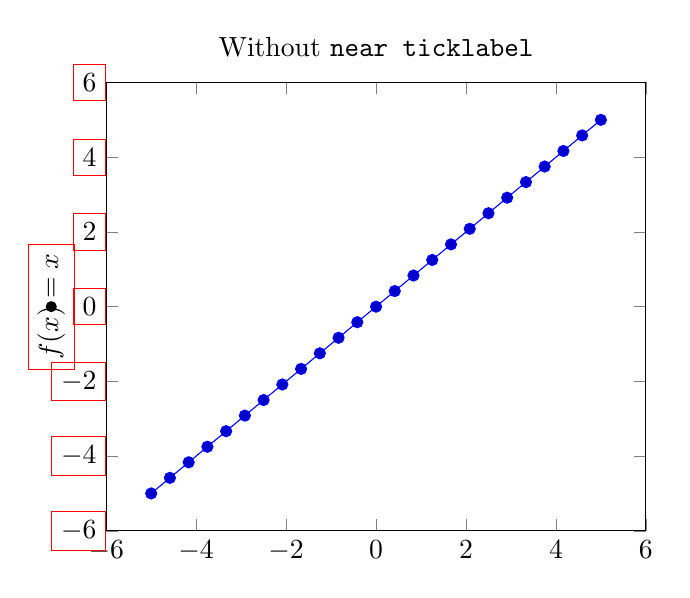
\begin{tikzpicture}
	\begin{axis}[
		title=Without \texttt{near ticklabel},
		ylabel={$f(x)=x$},
		every axis y label/.style=
			{at={(ticklabel cs:0.5)},rotate=90,anchor=center},
		clip=false,% to display the \path below
		ylabel style={draw=red},
		yticklabel style={draw=red}
	]

		\addplot {x};

		% visualize the position:
		\fill (yticklabel cs:0.5) circle(2pt);
	\end{axis}
\end{tikzpicture}%
~
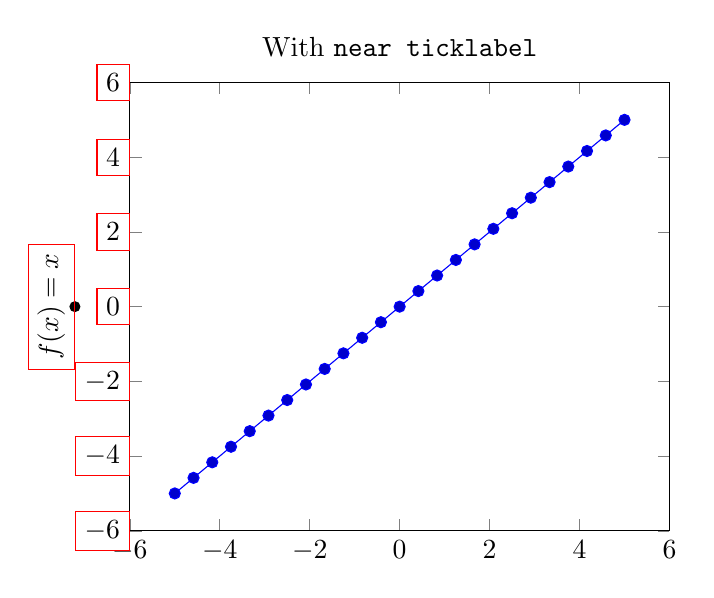
\begin{tikzpicture}
	\begin{axis}[
		title=With \texttt{near ticklabel},
		ylabel={$f(x)=x$},
		every axis y label/.style=
			{at={(ticklabel cs:0.5)},rotate=90,anchor=near ticklabel},
		clip=false,
		ylabel style={draw=red},
		yticklabel style={draw=red}
	]

		\addplot {x};
		\fill (yticklabel cs:0.5) circle(2pt);
	\end{axis}
\end{tikzpicture}
\end{document}
